\chapter{Game Examples}
\label{app:game-examples}

This appendix presents three notable game examples drawn directly from the Stockfish benchmark matches conducted during evaluation.
The games were selected to illustrate the range of the ResNet model's tactical capability: a swift, aggressive takedown of the (Elo~1320) preset, a grinding positional win against the near-Expert (Elo~2300) engine from the Black side, and the model's sole victory against the IM-strength (Elo~2800) preset.
All games were played search-less-the model selected moves in a single forward pass without any tree search-and were annotated with Stockfish centipawn evaluations at each ply.
The \texttt{[\%eval]} comments throughout each game reflect Stockfish's assessment of the position after the preceding move, expressed in pawns.

\begin{figure}[H]
    \centering
    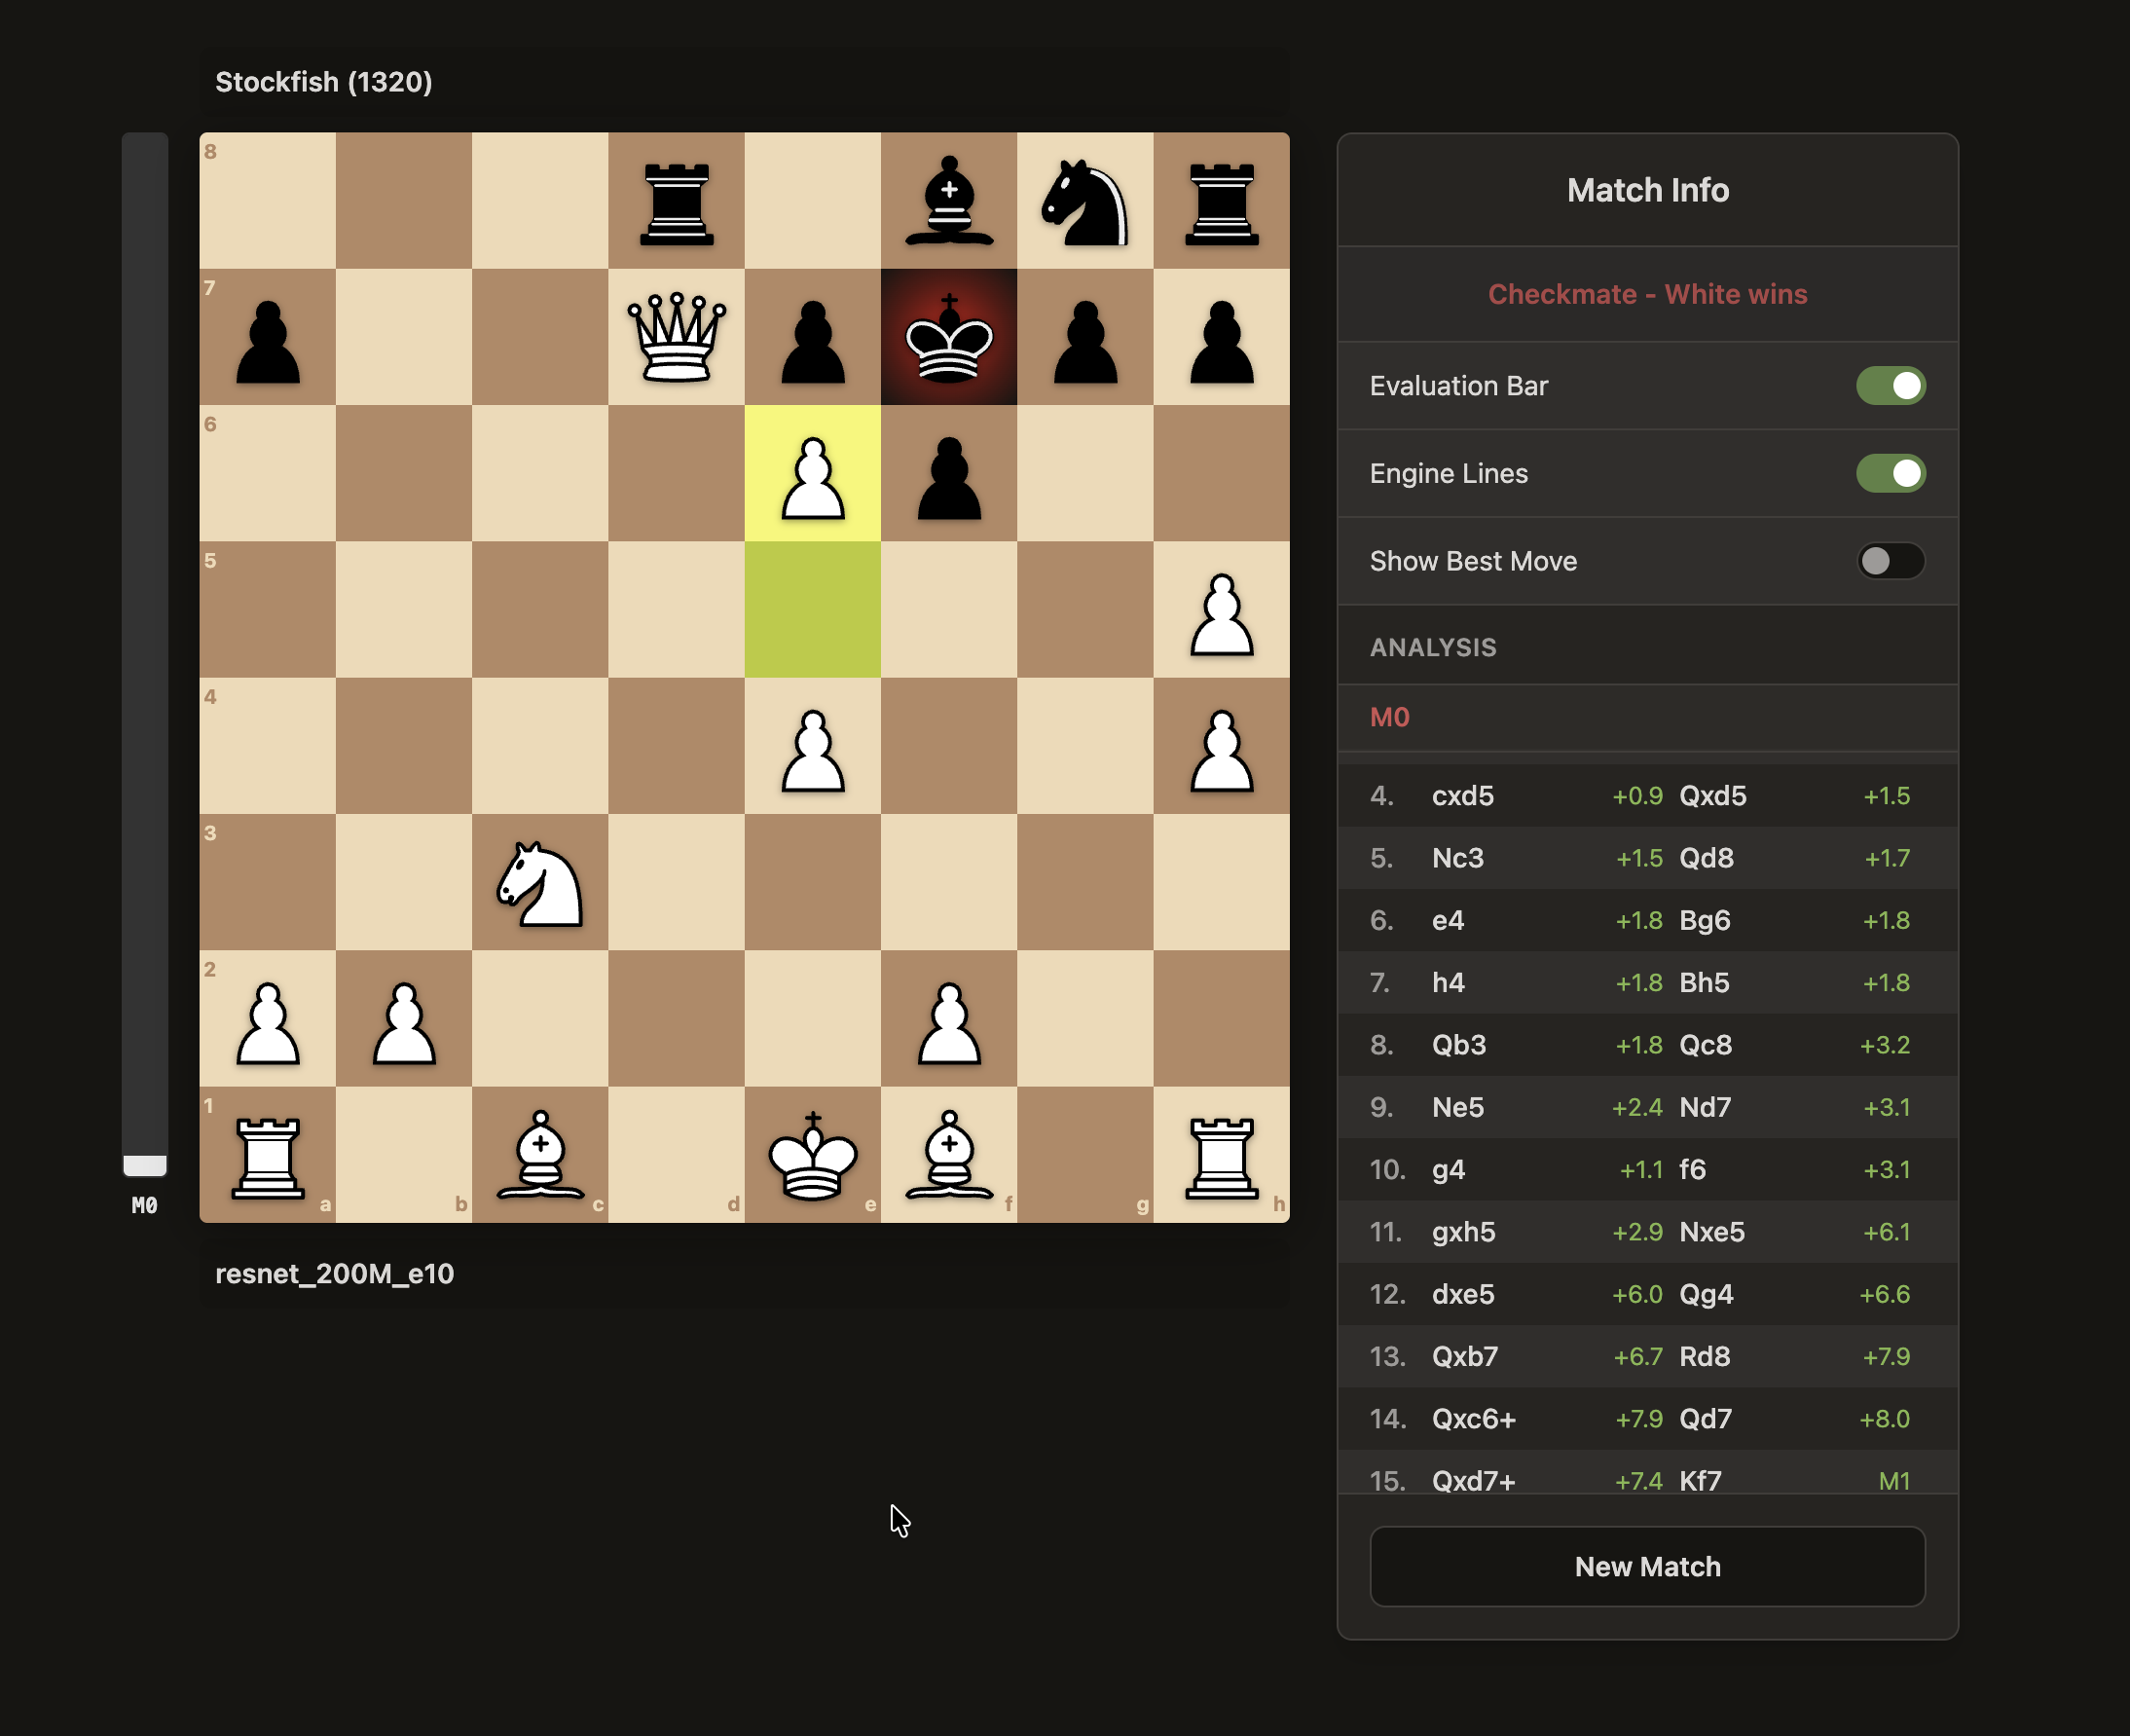
\includegraphics[width=0.7\linewidth]{figures/resnetwin.png}
    \caption{Final position of game played on the web interface between model and stockfish}
    \label{fig:resnetwin}
\end{figure}

% -------------------------

\section{Game 1: ResNet-200M vs 1320 Elo Stockfish}
\label{app:game1}

This game illustrates what happens when the ResNet model faces a low-strength Stockfish.
Playing White, the model opens with the English (\texttt{1.c4}) and immediately exerts pressure.
By move~10 Stockfish's position is already close to lost, and the game finishes with a composed back-rank checkmate (\texttt{18.Qxa8\#}) in just 18 move pairs.

\begin{verbatim}
[Event "resnet vs SF Novice-1320"]
[Site "?"]
[Date "2026.05.12"]
[Round "?"]
[White "ResNet_10B_256C"]
[Black "stockfish-ubuntu-x86-64-avxvnni_1320"]
[Result "1-0"]
[Termination "checkmate"]

1. c4 { [%eval 0.31] } 1... c6 { [%eval 0.48] } 
2. d4 { [%eval 0.45] } 2... d5 { [%eval 0.40] } 
3. Nf3 { [%eval 0.43] } 3... Be6 { [%eval 0.96] } 
4. cxd5 { [%eval 0.72] } 4... cxd5 { [%eval 0.74] } 
5. Nc3 { [%eval 0.66] } 5... Bf5 { [%eval 2.24] } 
6. Qb3 { [%eval 2.27] } 6... Nf6 { [%eval 2.17] } 
7. e4 { [%eval 2.29] } 7... dxe4 { [%eval 3.41] } 
8. Ne5 { [%eval 3.47] } 8... Qxd4 { [%eval 4.80] } 
9. Bf4 { [%eval 4.83] } 9... Nc6 { [%eval 5.09] } 
10. Qxb7 { [%eval 5.22] } 10... Nxe5 { [%eval 10.36] } 
11. Bb5+ { [%eval 11.02] } 11... Kd8 { [%eval 11.10] } 
12. Rd1 { [%eval 6.70] } 12... Qxd1+ { [%eval 8.13] }
13. Kxd1 { [%eval 8.76] } 13... e3 { [%eval 11.44] } 
14. Bxe5 { [%eval 98.40] } 14... e2+ { [%eval 99.40] } 
15. Kxe2 { [%eval 99.50] } 15... Bg4+ { [%eval 99.60] }
16. f3 { [%eval 99.70] } 16... g6 { [%eval 99.90] } 
17. Rd1+ { [%eval 99.90] } 17... Bd7 { [%eval 99.90] } 
18. Qxa8# { [%eval 0.00] } 1-0
\end{verbatim}

% -------------------------
\section{Game 2: ResNet-200M vs 2300 Elo Stockfish}
\label{app:game2}

Playing Black against Stockfish calibrated to 2300~Elo, the ResNet model builds a decisive positional advantage by move~17 and converts it to a forced checkmate by move~31.
The key moment happens at move~24 (\texttt{24\ldots Nxf3+}), where the model sacrifices a knight to strip away White's defensive pawn cover.
The game concludes with \texttt{31\ldots Rh2\#}.

\begin{verbatim}
[Event "resnet vs SF Expert-2300"]
[Site "?"]
[Date "2026.05.12"]
[Round "?"]
[White "stockfish-ubuntu-x86-64-avxvnni_2300"]
[Black "ResNet_10B_256C"]
[Result "0-1"]
[Termination "checkmate"]

1. d4 { [%eval 0.38] } 1... d5 { [%eval 0.40] } 
2. c4 { [%eval 0.33] } 2... e6 { [%eval 0.30] } 
3. g3 { [%eval 0.25] } 3... dxc4 { [%eval 0.26] } 
4. Nf3 { [%eval 0.21] } 4... a6 { [%eval 0.40] } 
5. Qc2 { [%eval -0.61] } 5... b5 { [%eval -0.51] } 
6. Bg5 { [%eval -0.52] } 6... Be7 { [%eval -0.48] } 
7. Bxe7 { [%eval -0.47] } 7... Nxe7 { [%eval -0.47] } 
8. e3 { [%eval -1.34] } 8... Bb7 { [%eval -1.37] } 
9. Nbd2 { [%eval -1.26] } 9... Nd7 { [%eval -1.29] } 
10. Bh3 { [%eval -1.99] } 10... c5 { [%eval -1.89] } 
11. O-O { [%eval -2.02] } 11... O-O { [%eval -1.87] } 
12. Rfd1 { [%eval -2.24] } 12... Nd5 { [%eval -2.04] } 
13. e4 { [%eval -2.02] } 13... Nb4 { [%eval -1.94] } 
14. Qc3 { [%eval -2.05] } 14... Nd3 { [%eval -1.63] } 
15. Bf1 { [%eval -2.87] } 15... cxd4 { [%eval -2.81] } 
16. Qa3 { [%eval -4.18] } 16... N7c5 { [%eval -3.84] } 
17. Nxc4 { [%eval -5.32] } 17... bxc4 { [%eval -5.24] } 
18. Bxd3 { [%eval -5.76] } 18... Nxd3 { [%eval -5.70] }
19. Nd2 { [%eval -5.94] } 19... Rc8 { [%eval -5.53] } 
20. Rf1 { [%eval -6.40] } 20... f5 { [%eval -4.99] } 
21. Nxc4 { [%eval -4.92] } 21... fxe4 { [%eval -5.63] }
22. Nd6 { [%eval -5.80] } 22... Qe7 { [%eval -5.57] } 
23. f3 { [%eval -6.62] } 23... Ne5 { [%eval -5.50] } 
24. Rae1 { [%eval -8.38] } 24... Nxf3+ { [%eval -9.05] }
25. Qxf3 { [%eval -9.24] } 25... exf3 { [%eval -9.19] } 
26. Nxc8 { [%eval -9.51] } 26... Rxc8 { [%eval -9.66] } 
27. a3 { [%eval -10.33] } 27... Rc2 { [%eval -12.64] }
28. h3 { [%eval -14.49] } 28... Qg5 { [%eval -99.60] } 
29. g4 { [%eval -99.60] } 29... Qh4 { [%eval -99.70] } 
30. b3 { [%eval -99.80] } 30... Qg3+ { [%eval -99.90] }
31. Kh1 { [%eval -99.90] } 31... Rh2# { [%eval 0.00] } 0-1
\end{verbatim}

% -------------------------
\section{Game 3: ResNet-200M's Sole Victory Against the IM Preset (Elo 2800)}
\label{app:game3}

Across the full benchmark, the ResNet model managed only one win against (Elo~2800) Stockfish.
The game follows a King's Indian Defence structure, and the model (White) builds a slow but relentless advantage during the match.
The evaluation gradually creeps from near-equal (\texttt{+0.29}) in the opening to a decisive \texttt{+6} around move~40.
The fact that the model achieves this without any lookahead-relying purely on learned policy-highlights how deeply the network has internalised strategic and tactical patterns from grandmaster games.

\begin{verbatim}
[Event "resnet vs SF IM-2800"]
[Site "?"]
[Date "2026.05.12"]
[Round "?"]
[White "ResNet_10B_256C"]
[Black "stockfish-ubuntu-x86-64-avxvnni_2800"]
[Result "1-0"]
[Termination "checkmate"]

1. c4 { [%eval 0.29] } 1... Nf6 { [%eval 0.35] } 
2. d4 { [%eval 0.34] } 2... c6 { [%eval 0.33] } 
3. Nc3 { [%eval 0.30] } 3... g6 { [%eval 0.77] } 
4. e4 { [%eval 0.88] } 4... d6 { [%eval 0.89] } 
5. Be2 { [%eval 0.84] } 5... Bg7 { [%eval 0.81] } 
6. Nf3 { [%eval 0.77] } 6... Na6 { [%eval 0.90] } 
7. O-O { [%eval 0.87] } 7... Bg4 { [%eval 1.18] } 
8. Be3 { [%eval 1.27] } 8... O-O { [%eval 1.22] } 
9. h3 { [%eval 1.27] } 9... Be6 { [%eval 1.60] } 
10. Qd2 { [%eval 1.55] } 10... Bd7 { [%eval 1.76] } 
11. Rad1 { [%eval 1.73] } 11... Nc7 { [%eval 1.70] } 
12. e5 { [%eval 1.73] } 12... Nfe8 { [%eval 1.75] } 
13. Rfe1 { [%eval 1.76] } 13... Bf5 { [%eval 1.86] } 
14. Qc1 { [%eval 1.71] } 14... b5 { [%eval 1.67] } 
15. b3 { [%eval 1.75] } 15... bxc4 { [%eval 1.76] } 
16. bxc4 { [%eval 1.72] } 16... d5 { [%eval 1.76] } 
17. Qa3 { [%eval 1.87] } 17... a5 { [%eval 1.89] } 
18. Rc1 { [%eval 1.73] } 18... Be6 { [%eval 2.14] } 
19. c5 { [%eval 1.78] } 19... f6 { [%eval 1.84] } 
20. Na4 { [%eval 1.86] } 20... fxe5 { [%eval 2.60] } 
21. Nxe5 { [%eval 1.65] } 21... Bxe5 { [%eval 1.73] } 
22. dxe5 { [%eval 1.73] } 22... d4 { [%eval 1.75] } 
23. Bh6 { [%eval 1.90] } 23... Rf7 { [%eval 2.21] } 
24. Nb6 { [%eval 2.27] } 24... Rb8 { [%eval 2.08] } 
25. Qa4 { [%eval 2.09] } 25... Ng7 { [%eval 2.25] } 
26. Qxc6 { [%eval 2.27] } 26... Bxa2 { [%eval 2.17] } 
27. Qa4 { [%eval 2.33] } 27... Be6 { [%eval 2.25] } 
28. Qxa5 { [%eval 1.58] } 28... Nd5 { [%eval 1.63] } 
29. Rb1 { [%eval 1.11] } 29... Nc3 { [%eval 1.08] } 
30. Rb2 { [%eval 1.12] } 30... Rf8 { [%eval 2.57] } 
31. Bd3 { [%eval 2.51] } 31... Bxh3 { [%eval 3.08] } 
32. gxh3 { [%eval 3.56] } 32... e6 { [%eval 3.84] } 
33. Qa7 { [%eval 3.02] } 33... Rf7 { [%eval 3.08] } 
34. Qa6 { [%eval 3.12] } 34... Qe7 { [%eval 5.58] } 
35. c6 { [%eval 3.45] } 35... Ne8 { [%eval 4.20] }
36. Qc4 { [%eval 4.43] } 36... Rf3 { [%eval 5.09] } 
37. Bf1 { [%eval 5.37] } 37... Nc7 { [%eval 5.68] } 
38. Bg2 { [%eval 5.14] } 38... Qh4 { [%eval 5.44] } 
39. Bxf3 { [%eval 5.69] } 39... Qxh6 { [%eval 5.89] } 
40. Qxd4 { [%eval 5.84] } 40... N7b5 { [%eval 6.08] } 
41. Qe3 { [%eval 6.21] } 41... Qh4 { [%eval 6.40] } 
42. Bg2 { [%eval 6.43] } 42... Qd8 { [%eval 7.19] } 
43. Nd7 { [%eval 7.58] } 43... Rc8 { [%eval 8.06] } 
44. Qc5 { [%eval 7.35] } 44... Qg5 { [%eval 7.61] }
45. Rxb5 { [%eval 8.49] } 45... Nxb5 { [%eval 9.97] } 
46. Qxb5 { [%eval 8.08] } 46... Kh8 { [%eval 10.84] } 
47. Qb7 { [%eval 8.22] } 47... Qd8 { [%eval 8.56] } 
48. Rd1 { [%eval 7.77] } 48... g5 { [%eval 12.86] } 
49. Bf3 { [%eval 11.41] } 49... h5 { [%eval 99.30] } 
50. Nf6 { [%eval 99.40] } 50... Qxf6 { [%eval 99.70] } 
51. exf6 { [%eval 99.80] } 51... e5 { [%eval 99.90] }
52. Qg7# { [%eval 0.00] } 1-0
\end{verbatim}
